\documentclass{article}
\usepackage[T1]{fontenc}
\usepackage{lmodern}
\usepackage{graphicx}
\usepackage{amsmath,amssymb}
\usepackage[a4paper,margin=2cm]{geometry}
\usepackage[absolute,overlay]{textpos}
\setlength{\TPHorizModule}{1mm}
\setlength{\TPVertModule}{1mm}
\usepackage[indonesian]{babel}
\usepackage{hyperref}
\setlength{\emergencystretch}{2em}
% unit: Halaman 43

\begin{document}

% === Halaman 43 (llm) ===

\vspace{234.63mm}

\section*{Vigenere Cipher dalam Python}

% deskripsi: Screenshot kode program Python untuk fungsi enkripsi Vigenere Cipher (Vigenere\_cipher\_encrypt) dan dekripsi (Vigenere\_cipher\_decrypt).
% bbox normalisasi: [0.0000, 0.1200, 0.8000, 0.9100]
\begin{textblock*}{168.00mm}(0.00mm,35.64mm)
\noindent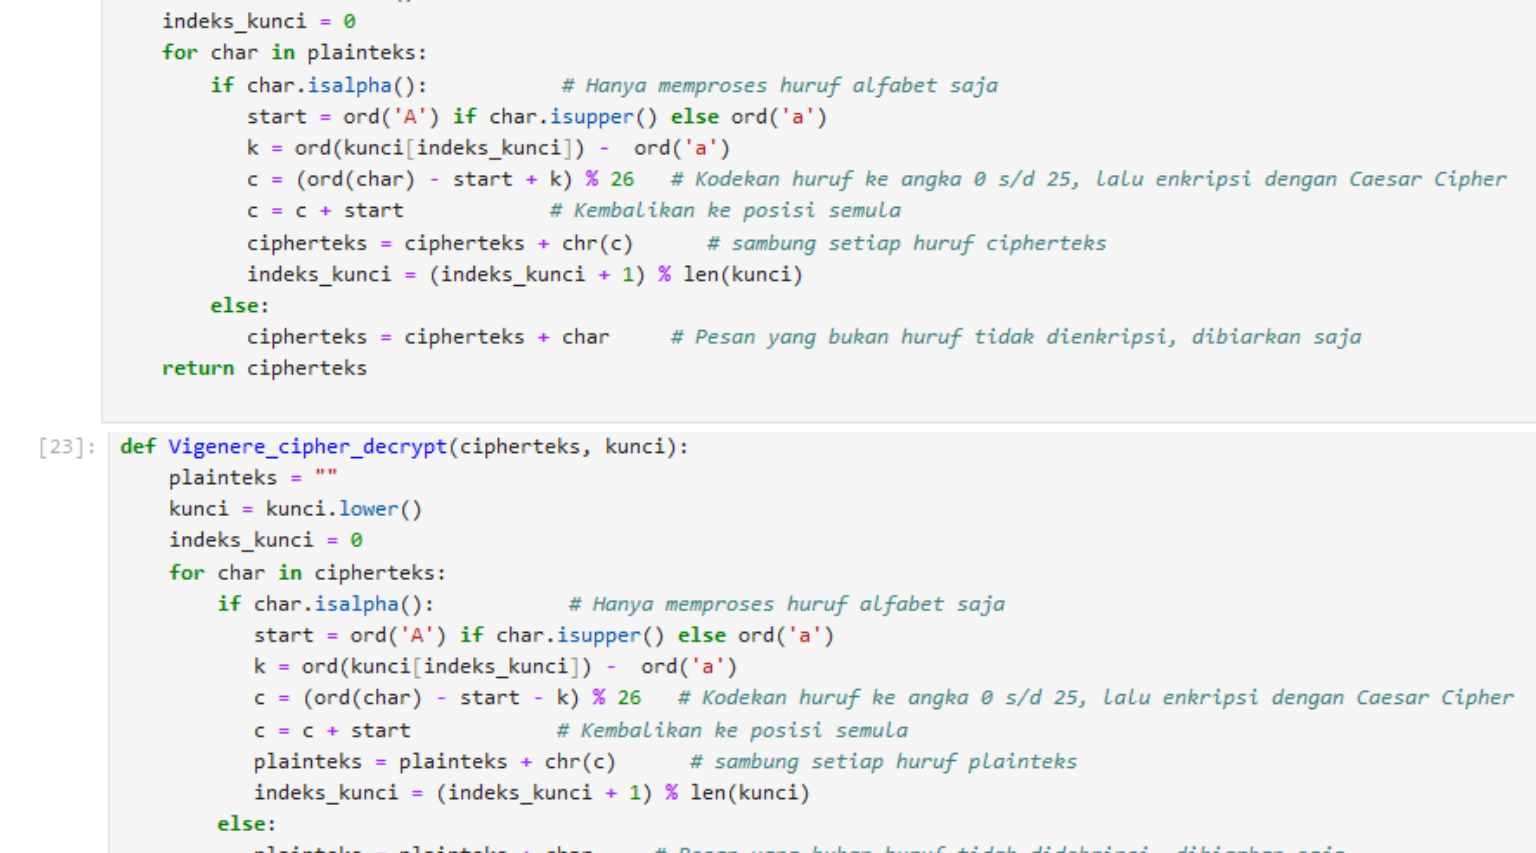
\includegraphics[width=168.00mm,height=234.63mm]{../../images/llm/page_043_img_01.png}%
\end{textblock*}

\end{document}
